\fig{fv:e3:power}{同一杆内力可以分别做功，总功率由沿杆相对速度决定}{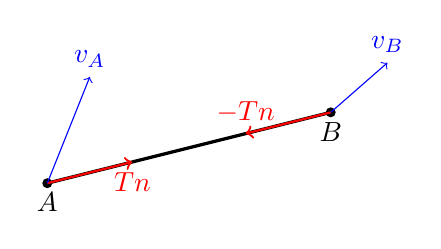
\begin{tikzpicture}[scale=.9]
\coordinate(A)at(0,0);\coordinate(B)at(4,1);\draw[very thick](A)--(B);\fill(A)circle(2pt)node[below]{$A$};\fill(B)circle(2pt)node[below]{$B$};
\draw[->,red,thick](A)--(1.2,.3)node[below]{$T\bm n$};\draw[->,red,thick](B)--(2.8,.7)node[above]{$-T\bm n$};
\draw[->,blue](A)--(.6,1.5)node[above]{$\bm v_A$};\draw[->,blue](B)--(4.8,1.7)node[above]{$\bm v_B$};
\end{tikzpicture}}
图\ref{fv:e3:power}的杆长条件限制的是 $(\bm v_A-\bm v_B)\cdot\bm n=0$。两端内力的总功率因而为零，尽管各自与端点速度的点积不必为零。若杆可伸长，这个投影一般不再为零，内力便可改变弹性储能。讨论“内力是否做功”之前，必须先明确说的是某一端的功，还是整个固定物质系统内力的总功。
